\chapter{Dataset}\label{chap:dataset}

\section{electronic Intensive Care Unit}\label{sec:eicu}

\acrfull{eICU-CRD} Version 2.0 is an open access, multicenter critical care database published by Philips Healthcare in partnership with the MIT \acrfull{LCP}. It contains data of 200,859 ICU admissions for 139,367 unique patients in 208 hospitals across the United States. The data were employed from 2014 and 2015 \cite{cosgriff_developing_2019}, but it has been publicly available\footnote{\href{https://eicu-crd.mit.edu/}{https://eicu-crd.mit.edu/}} since April 2019. \acrshort{eICU} includes 31 tables that can be categorized into five different divisions based on types of data: \

\begin{itemize}
    \item care documentation
    \item \acrshort{APACHE}
    \item care plan
    \item administration
    \item monitor data
\end{itemize}

{\hskip 1em} An informative summary of these tables is shown in table \ref{tab:maindemo}. All tables are related to each other, except \textit{hospital}, using an identifier called {\small\fontfamily{pcr}\selectfont{patientunitstayid}}. Generally, there are three identifiers in \acrshort{eICU}:

\begin{itemize}
    \item {\small\fontfamily{pcr}\selectfont{patientunitstayid}}
    \item {\small\fontfamily{pcr}\selectfont{patienthealthsystemstayid}}
    \item {\small\fontfamily{pcr}\selectfont{uniquepid}}
\end{itemize}

{\hskip 1em} How these identifiers are related is illustrated in figure \ref{fig:eicuidentifiers}. The figure demonstrates that each {\small\fontfamily{pcr}\selectfont{patienthealthsystemstayid}} has at least one or more {\small\fontfamily{pcr}\selectfont{patientunitstayid}}, and each {\small\fontfamily{pcr}\selectfont{uniquepid}} can have multiple {\small\fontfamily{pcr}\selectfont{patienthealthsystemstayid}} or {\small\fontfamily{pcr}\selectfont{patientunitstayid}}. An example of such relations can be seen in figure \ref{fig:patienttable}, where the patient has one  {\small\fontfamily{pcr}\selectfont{uniquepid}} with two {\small\fontfamily{pcr}\selectfont{patienthealthsystemstayid}}s and four different {\small\fontfamily{pcr}\selectfont{patientunitstayid}}s.

\begin{table}[!htbp]
\centering
\setlength\tabcolsep{15pt}
\caption{\label{tab:maindemo}Summary of available measurements for the two versions of the \acrshort{eICU-CRD}}
\resizebox{0.87\textwidth}{!}{%
\begin{tabular}{@{}llll@{}}
\toprule
\thead{Table} & \thead{No. of Columns} & \thead{Demo Version Rows} & \thead{Main Version Rows} \\ \midrule \midrule
admissionDrug               & 14    & 7,417     & 874,920       \\ \midrule
admissionDx                 & 6     & 7,578     & 626,858       \\ \midrule
allergy                     & 13    & 2,475     & 251,949       \\ \midrule
apacheApsVar                & 26    & 2,205     & 171,177       \\ \midrule
apachePatientResult         & 23    & 3,676     & 297,064       \\ \midrule
apachePredVar               & 51    & 2,205     & 171,177       \\ \midrule
carePlanCareProvider        & 8     & 5,627     & 502,765       \\ \midrule
carePlanEOL                 & 5     & 15        & 1,433         \\ \midrule
carePlanGeneral             & 6     & 33,148    & 3,115,018     \\ \midrule
carePlanGoal                & 7     & 3,633     & 504,139       \\ \midrule
carePlanInfectiousDisease   & 8     & 112       & 8,056         \\ \midrule
customLab                   & 7     & 30        & 1,082         \\ \midrule
diagnosis                   & 7     & 24,978    & 2,710,672     \\ \midrule
hospital                    & 4     & 186       & 208           \\ \midrule
infusionDrug                & 9     & 38,256    & 4,803,719     \\ \midrule
intakeOutput                & 12    & 100,466   & 12,030,289    \\ \midrule
lab                         & 10    & 434,660   & 39,132,531    \\ \midrule
medication                  & 15    & 75,604    & 7,301,853     \\ \midrule
microLab                    & 7     & 342       & 16,996        \\ \midrule
note                        & 8     & 24,758    & 2,254,179     \\ \midrule
nurseAssessment             & 8     & 91,589    & 15,602,498    \\ \midrule
nurseCare                   & 8     & 42,080    & 8,311,132     \\ \midrule
nurseCharting               & 8     & 1,477,163 & 151,604,232   \\ \midrule
pastHistory                 & 8     & 12,109    & 1,149,180     \\ \midrule
patient                     & 29    & 2,520     & 200,859       \\ \midrule
physicalExam                & 6     & 84,058    & 9,212,316     \\ \midrule
respiratoryCare             & 34    & 5,436     & 865,381       \\ \midrule
respiratoryCharting         & 7     & 176,089   & 20,168,176    \\ \midrule
treatment                   & 5     & 38,290    & 3,688,745     \\ \midrule
vitalAperiodic              & 13    & 274,088   & 25,075,074    \\ \midrule
vitalPeriodic               & 19    & 1,634,960 & 146,671,642   \\ \midrule
                                                                \\
\textbf{31 Tables} & \textbf{391}  & \textbf{4,605,753} & \textbf{457,325,320} \\ \midrule
\textbf{No. of Unique Patients} &  & \textbf{1,841}     & \textbf{139,367} \\
\bottomrule
\end{tabular}}
\end{table}

\begin{figure}[ht]
\centering
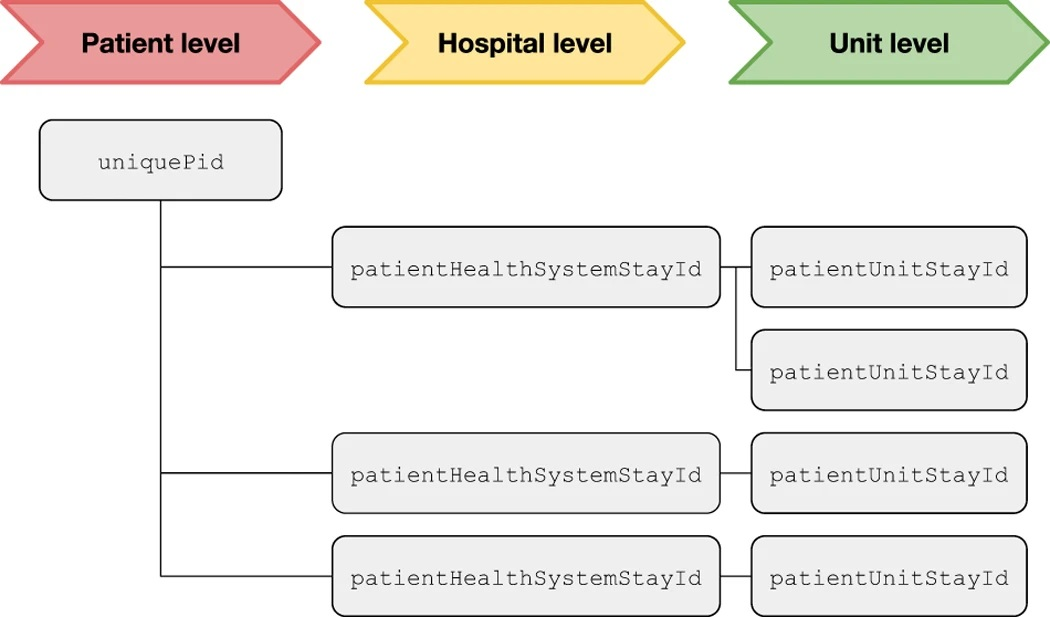
\includegraphics[width=14cm]{fig/chapter3/Organization of patient tracking information.jpg}
\caption{Organization of patient tracking information \cite{pollard_eicu_2018}}
\label{fig:eicuidentifiers}
\end{figure}

\begin{figure}[ht]
\centering
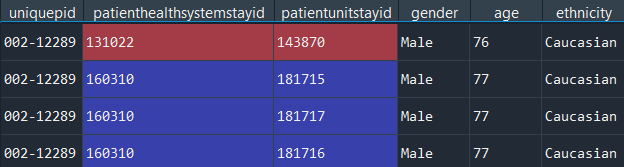
\includegraphics[width=14cm]{fig/chapter3/patient_mod.png}
\caption{Different patient identifiers in \textit{patient} table of the \acrshort{eICU-CRD}}
\label{fig:patienttable}
\end{figure}

\subsection{eICU Demo Version}

The demo version of the \acrshort{eICU} is publicly available after creating an account on the PhysioNet repository\footnote{\href{https://physionet.org/content/eicu-crd-demo/2.0/}{https://physionet.org/content/eicu-crd-demo/2.0/}}. It can be a good practice of getting to know the database, its tables, and their features before switching into the main database for our final cohort approach. In the following, the relevant tables to our goal are introduced briefly.

\subsubsection{\textit{admissionDrug}}
The table includes medication details of a patient prior to their \acrshort{ICU} admission. Since Greco et al. in \cite{greco_diabetes_2018} hypothesized that \acrshort{DM} might influence the association of hyperlactatemia with in-hospital mortality, this work is interested in separating patients who have diabetes or use drugs for glycemic control. A list of anti-diabetic medications (hereafter drug list) and their corresponding \acrshort{HICL} sequence numbers was extracted in this regard. Figure \ref{fig:admissiondrug} shows the most important parameters/columns of the \textit{admissionDrug} table for our study for a single patient. This table has the information of 449 patients (amid overall 1841 patients in the demo version of the \acrshort{eICU}), and 143 of them have the satisfying condition of the drug list.

\begin{figure}[ht]
\centering
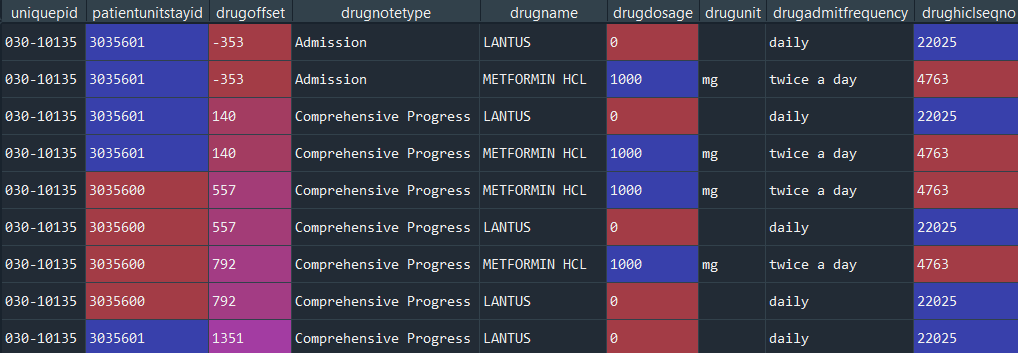
\includegraphics[width=15cm]{fig/chapter3/admissiondrug_m.png}
\caption{A slice of the \textit{admissionDrug} table for a unique patient}
\label{fig:admissiondrug}
\end{figure}

\subsubsection{\textit{admissionDx}}
This table contains the primary diagnosis for the ICU admission per the APACHE scoring criteria. This means that if a patient does not have an \textit{admissionDx} entry, they could not have an \acrshort{APACHE} score. Among 1777 patients in this table, only 145 of them were diagnosed to have a diabetic disease. Figure \ref{fig:admissiondx} shows a part of a unique patient's information in the \textit{admissionDx}.

\begin{figure}[ht]
\centering
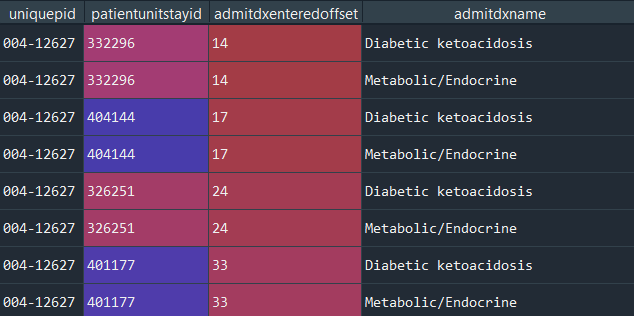
\includegraphics[width=15cm]{fig/chapter3/admissiondx_m.png}
\caption{A slice of the \textit{admissionDx} table for a unique patient}
\label{fig:admissiondx}
\end{figure}

\subsubsection{\textit{allergy}}
The \textit{allergy} table includes patients' allergies in detail. Out of 589 unique patients in this table, only ten patients have been admitted to the \acrshort{ICU} with diabetic-related allergies. A sample of the \textit{allergy} table is shown in figure \ref{fig:allergy}.

\begin{figure}[ht]
\centering
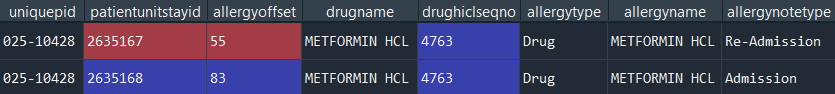
\includegraphics[width=15cm]{fig/chapter3/allergy_m.png}
\caption{A slice of the \textit{allergy} table for a unique patient}
\label{fig:allergy}
\end{figure}

\subsubsection{\textit{apacheApsVar}}
This table is the first amongst the three \acrshort{APACHE} tables in the \acrshort{eICU-CRD}. It contains the required variables for the calculation of \acrfull{APS}-III for patients in the first 24 hours of their \acrshort{ICU} admissions. The \textit{apacheApsVar} table contains information about 1786 patients, one of which can be seen in figure \ref{fig:apacheapsvar}. 

\begin{figure}[ht]
\centering
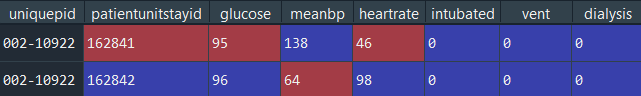
\includegraphics[width=15cm]{fig/chapter3/apacheapsvar.png}
\caption{A slice of the \textit{apacheApsVar} table for a unique patient}
\label{fig:apacheapsvar}
\end{figure}

\subsubsection{\textit{apachePatientResult}}
The \textit{apachePatientResult} table provides predictions made by the \acrshort{APACHE} score in both versions (IV and IVa) for each patient. As demonstrated in figure \ref{fig:apachepatientresult}, {\small\fontfamily{pcr}\selectfont{actualicumortality}} is a unit disposition, while {\small\fontfamily{pcr}\selectfont{actualhospitalmortality}} is a hospital disposition; each can be either EXPIRED or ALIVE. {\small\fontfamily{pcr}\selectfont{actualhospitalmortality}} is considered as the final discharge status of a patient. As of this table's provided information, there are 1512 patients out of whom 129 have the expired hospital discharge status.

\begin{figure}[ht]
\centering
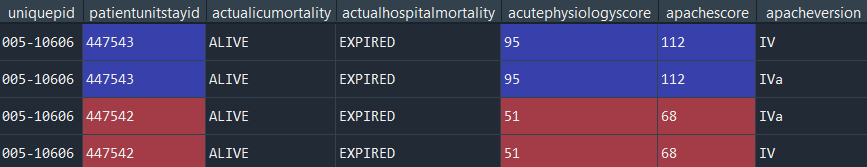
\includegraphics[width=15cm]{fig/chapter3/apachepatientresult.png}
\caption{A slice of the \textit{apachePatientResult} table for a unique patient}
\label{fig:apachepatientresult}
\end{figure}

\subsubsection{\textit{apachePredVar}}
The last \acrshort{APACHE} table provides variables underlying the APACHE predictions. In this table, {\small\fontfamily{pcr}\selectfont{gender}} 0 indicates Male, while {\small\fontfamily{pcr}\selectfont{gender}} 1 indicates Female. Furthermore, as it is seen in {\small\fontfamily{pcr}\selectfont{actualhospitalmortality}} in the \textit{apachePatientResult} table, there is a column named {\small\fontfamily{pcr}\selectfont{diedinhospital}} that is equal to the EXPIRED status in {\small\fontfamily{pcr}\selectfont{actualhospitalmortality}} when it is 1. For instance, the last row in figure \ref{fig:apachepredvar} shows that the patient with the unique patient id of 027-105179 who had diabetes, passed away one year after his (considering {\small\fontfamily{pcr}\selectfont{gender}}) admission to \acrshort{ICU}. Concerning this table, there are 369 diabetic patients, 179 EXPIRED ones, and 27 in common.

\begin{figure}[ht]
\centering
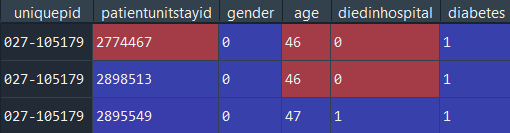
\includegraphics[width=15cm]{fig/chapter3/apachepredvar.png}
\caption{A slice of the \textit{apachePredVar} table for a unique patient}
\label{fig:apachepredvar}
\end{figure}

\subsubsection{\textit{diagnosis}}
Active patient diagnosis is recorded in the \textit{diagnosis} table, unlike the \textit{admissionDx} table with the diagnosis at admission time. There are 1709 unique patients in this table, out of whom 291 patients fulfill the drug list condition. As shown in figure \ref{fig:diagnosis}, the \textit{diagnosis} table is an explanatory one that can be used for patient stratification.

\begin{figure}[ht]
\centering
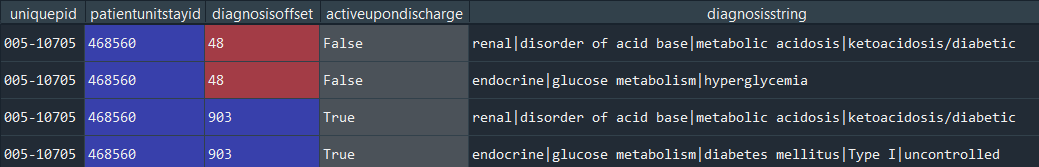
\includegraphics[width=15cm]{fig/chapter3/diagnosis_m.png}
\caption{A slice of the \textit{diagnosis} table for a unique patient}
\label{fig:diagnosis}
\end{figure}

\subsubsection{\textit{infusionDrug}}
The \textit{infusionDrug} table has the drug infusions in detail, including concentration ({\small\fontfamily{pcr}\selectfont{drugamount}}) and how the drug should be administered. It also contains {\small\fontfamily{pcr}\selectfont{patientweight}}, which is used further to complete our dataset when a weight value from the \textit{patient} table is missing. Figure \ref{fig:infusiondrug} shows part of this table.

\begin{figure}[ht]
\centering
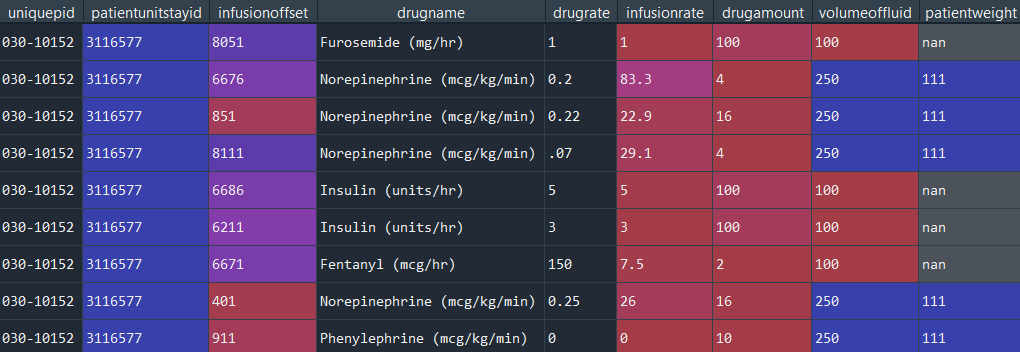
\includegraphics[width=15cm]{fig/chapter3/infusiondrug.png}
\caption{A slice of the \textit{infusionDrug} table for a unique patient}
\label{fig:infusiondrug}
\end{figure}

\subsubsection{\textit{intakeOutput}}
This table comprises of recorded intake or output of any volume for patients. For our purpose, the only record that is of interest in the \textit{intakeOutput} table (as in figure \ref{fig:intakeoutput}) is insulin, which is available for 69 patients among a total of 1633 patients in this table.

\begin{figure}[ht]
\centering
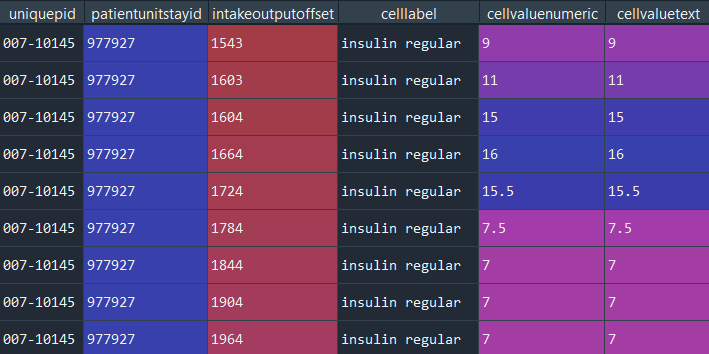
\includegraphics[width=15cm]{fig/chapter3/intakeoutput_m.png}
\caption{A slice of the \textit{intakeOutput} table for a unique patient}
\label{fig:intakeoutput}
\end{figure}

\subsubsection{\textit{lab}}
The \textit{lab} table is essential for our study. It includes all the laboratory tests for a patient collected during his/her stay in the hospital. Although there is a total of 158 distinct types of laboratory measurements \cite{pollard_eicu_2018}, regarding our objective, we are interested in just three types of measurements (see figure \ref{fig:lab}): \

\begin{itemize}
    \item glucose
    \item bedside glucose
    \item lactate
\end{itemize}

{\hskip 1em} Note that the \textit{lab} table is the only table with lactate measurement amid all the 31 tables of the \acrshort{eICU}. \

\begin{figure}[ht]
\centering
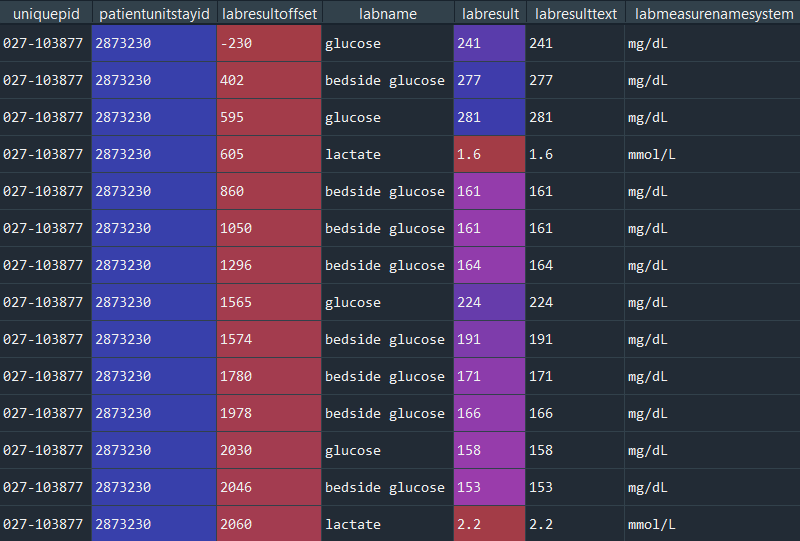
\includegraphics[width=15cm]{fig/chapter3/lab_m.png}
\caption{A slice of the \textit{lab} table for a unique patient}
\label{fig:lab}
\end{figure}

{\hskip 1em} Almost all the patients have lab measurements (1826 out of 1841), and among them, 1803 patients have at least one of the three aforementioned measurement types. The distribution of each is demonstrated in table \ref{tab:labtabledist}.

\begin{table}[h]
\centering
\setlength\tabcolsep{60pt}
\caption{\label{tab:labtabledist}Distribution of lactate and glucose measurements in the \textit{lab} table}
\begin{tabular}{@{}rc@{}}
\toprule
\thead{Measurement}            & \thead{No. of Patients} \\ \midrule \midrule
\textbf{glucose}               & 857                     \\ \midrule
\textbf{bedside glucose}       & 1245                    \\ \midrule
\textbf{lactate}               & 811                     \\
\bottomrule
\end{tabular}
\end{table}

{\hskip 1em} Since lactate is one of the crucial elements needed for our dataset, a maximum of 811 patients from the \textit{lab} table can be used should those patients have glucose measurements as well.

\subsubsection{\textit{medication}}
The \textit{medication} table consists of active medication orders for patients. However, these orders might not necessarily be administered, and the table does not provide information in this regard. The information of 1372 patients is available in this table, while 826 of them have our desired drug list expectation. Take into consideration that  {\small\fontfamily{pcr}\selectfont{\acrfull{PRN}}} is a Latin phrase that means "as needed." This indicates that it is meaningful as long as {\small\fontfamily{pcr}\selectfont{\acrshort{PRN}}} is set to YES, which is in line with the {\small\fontfamily{pcr}\selectfont{frequency}}.

\begin{figure}[ht]
\centering
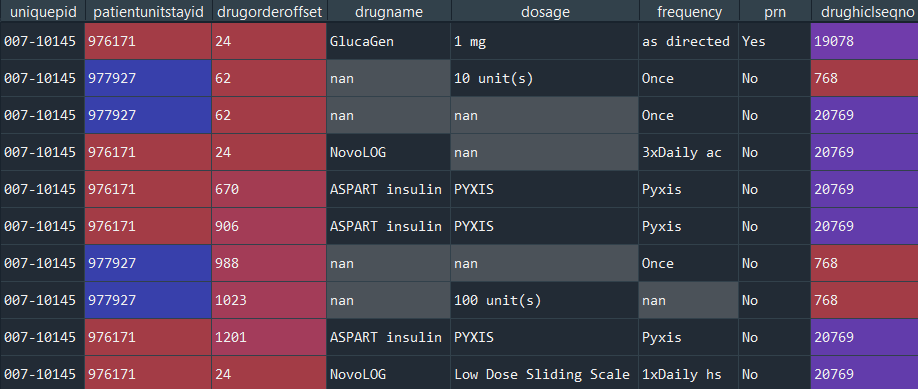
\includegraphics[width=15cm]{fig/chapter3/medication_m.png}
\caption{A slice of the \textit{medication} table for a unique patient}
\label{fig:medication}
\end{figure}

\subsubsection{\textit{nurseCharting}}
The \textit{nurseCharting} table is a nurse-entered information table in which, based on our needed values, it just has bedside glucose measurements. The number of such measurements is available for 481 out of 1786 patients. Part of this table is shown in figure \ref{fig:nursechart}.

\begin{figure}[ht]
\centering
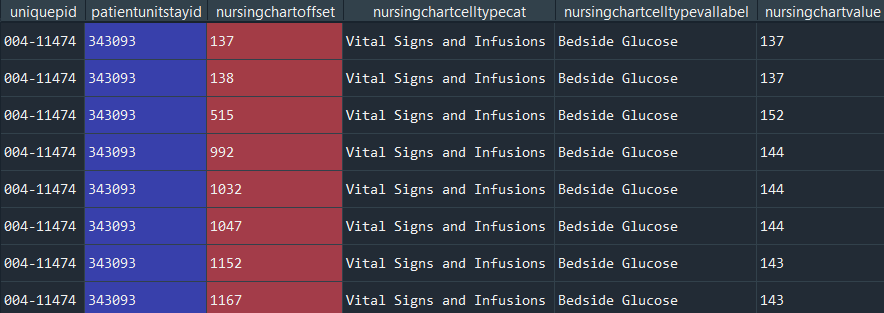
\includegraphics[width=15cm]{fig/chapter3/nursechart_m.png}
\caption{A slice of the \textit{nurseCharting} table for a unique patient}
\label{fig:nursechart}
\end{figure}

\subsubsection{\textit{pastHistory}}
All the relevant information related to the past medical history of a patient is stored in the \textit{pastHistory} table. It contains 1771 patients' information, 509 of them are of our interest, including all the 369 diabetic patients previously described in the \textit{apachePredVar} table.

\begin{figure}[H]
\begin{tabular}{@{}c@{}}
\begin{subfigure}{1\textwidth}
  \centering
  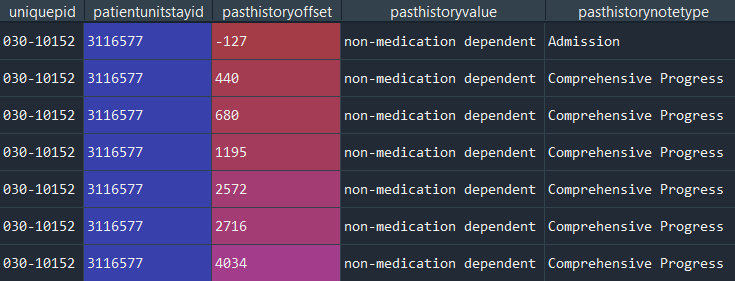
\includegraphics[width=15cm]{fig/chapter3/pasthistory_m1.png}
  \caption{\footnotesize{A patient who has diabetes type II, non-medication dependent}}
  \label{fig:pasthisotory1}
\end{subfigure} \\
\begin{subfigure}{1\textwidth}
  \centering
  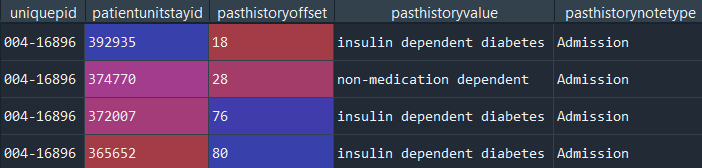
\includegraphics[width=15cm]{fig/chapter3/pasthistory_m2.png}
  \caption{\footnotesize{A patient who has diabetes type I, insulin-dependent and diabetes type II, non-medication dependent}}
  \label{fig:pasthisotory2}
\end{subfigure} \\
\begin{subfigure}{1\textwidth}
  \centering
  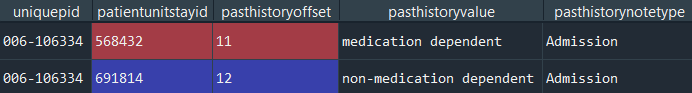
\includegraphics[width=15cm]{fig/chapter3/pasthistory_m3.png}
  \caption{\footnotesize{A patient who has diabetes type II, both medication and non-medication dependent}}
  \label{fig:pasthisotory3}
\end{subfigure} \\
\begin{subfigure}{1\textwidth}
  \centering
  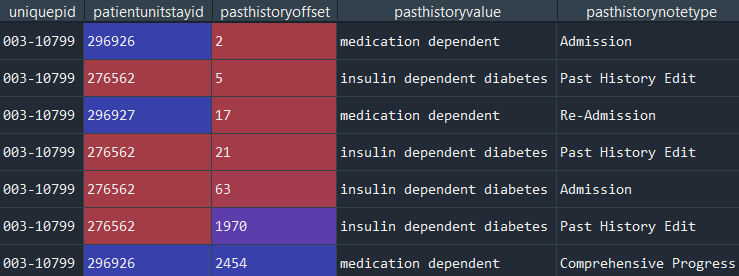
\includegraphics[width=15cm]{fig/chapter3/pasthistory_m4.png}
  \caption{\footnotesize{A patient who has diabetes type I, insulin-dependent and diabetes type II, medication dependent}}
  \label{fig:pasthisotory4}
\end{subfigure} \\
\end{tabular}
\caption{A slice of the \textit{pastHistory} table for four different diabetic patients}
\label{fig:pasthisotory}
\end{figure}

{\hskip 1em} There are two types of diabetes, diabetes type I (insulin-dependent) and diabetes type II (non-insulin-dependent), divided into two subgroups: medication dependent and non-medication dependent. As shown in figure \ref{fig:pasthisotory}, there are some intersections between these types for a unique patient. Table \ref{tab:diabeticdist} represents the distribution of the different types of diabetic patients and the number of intersections in the \textit{pastHistory} table.

\begin{table}[ht]
\centering
\setlength\tabcolsep{10pt}
\caption{\label{tab:diabeticdist}Distribution of the different types of diabetic patients}
\resizebox{0.95\textwidth}{!}{%
\begin{tabular}{@{}cccc@{}}
\toprule
\multirow{2}{*}{\thead{Diabetes}} & \thead{Type I} & \thead{Type II} & \thead{Type II} \\
& \thead{Insulin-dependent} & \thead{Medication dependent} & \thead{Non-medication dependent} \\ \midrule \midrule
\textbf{Type I}             & \multirow{2}{*}{216}    & \multirow{2}{*}{34}     & \multirow{2}{*}{3}       \\ 
\textbf{Insulin-dependent}  \\ \midrule
\textbf{Type II}                   & \multirow{2}{*}{34}     & \multirow{2}{*}{239}    & \multirow{2}{*}{6}     \\
\textbf{Medication dependent} \\ \midrule
\textbf{Type II} & \multirow{2}{*}{3} & \multirow{2}{*}{6} & \multirow{2}{*}{54}\\
\textbf{Non-medication dependent} \\
\bottomrule
\end{tabular}}
\end{table}

\subsubsection{\textit{patient}}
The \textit{patient} table includes patient demographic information and admission/discharge details during hospitalization. As discussed earlier in section \ref{sec:eicu}, all three patient identifiers were contained only in this table. The cohort selection of our work is started by patient stratification using the \textit{patient} table.

\subsubsection{\textit{treatment}}
Our study's last useful table is the \textit{treatment} table, which contains the patient's active treatments. There are 1518 patients in this table, out of whom 333 are of interest to the investigation based on the drug list. Figure \ref{fig:treatment} shows part of this table for a single patient.

\begin{figure}[ht]
\centering
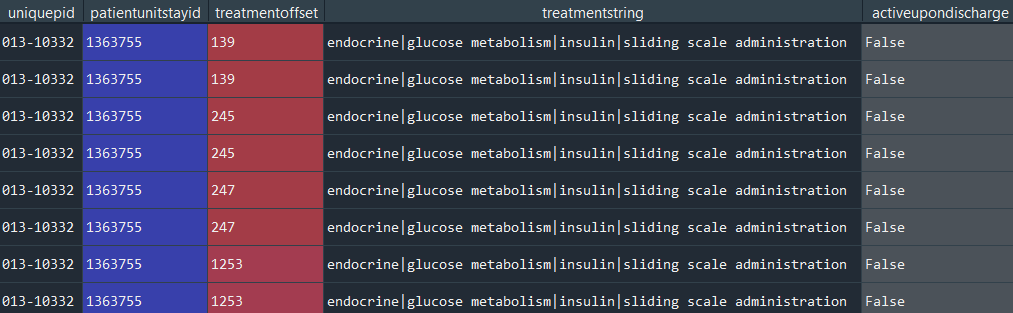
\includegraphics[width=15cm]{fig/chapter3/treatment_m.png}
\caption{A slice of the \textit{treatment} table for a unique patient}
\label{fig:treatment}
\end{figure}

\subsection{eICU Main Version}
In order to have access to the main version of the \acrshort{eICU}, one needs to complete the \acrshort{CITI} “Data or Specimens Only Research” course. Once the application completion is approved, the \acrshort{eICU-CRD} main version (Version 2.0) is accessible via PhysioNet repository\footnote{\href{https://physionet.org/content/eicu-crd/2.0/}{https://physionet.org/content/eicu-crd/2.0/}}. A brief comparison of the two versions of the \acrshort{eICU} was given in table \ref{tab:maindemo}. The main version has the exact 31 tables as in the demo version but with a factor of nearly 80 times the number of patients contained in the demo version, and hence, measurements. Having such a massive size of over 457 million rows of measurements sets some limitations in thoroughly analyzing this database as presented for its demo version using a local computer. Therefore, the \acrfull{HUNT} Cloud service was used, which had its own drawbacks. All of these limitations will be discussed in section \ref{ssec:limit}. However, the \acrshort{eICU-CRD} main version is our principal database for further analysis. 

\section{Cohort Selection}
Amongst all the 31 tables, 391 columns, and 457,325,320 rows of the \acrshort{eICU} database, we need to extract a cohort for the implementation. In this regard, first, it is necessary to select the related features to our goal. As we seek the association of glucose and lactate with mortality, both are chosen to build our dataset. Besides these two variables, we are interested in finding the importance of some demographic information, such as age, gender, and weight. Furthermore, considering the conducted survey of Greco et al. \cite{greco_diabetes_2018}, we select diabetes as one of our features to deepen our study. All in all, our ideal dataset consists of 139,367 rows (number of patients) and six columns as the following:

\begin{itemize}
    \item age
    \item gender
    \item weight
    \item glucose level
    \item lactate level
    \item diabetes
\end{itemize}

{\hskip 1em} To add more details to our study, weight is replaced by admission weight and discharge weight. Moreover, unlike the glucose level that can be found in various tables (e.g., \textit{apacheApsVar}, \textit{lab}, \textit{medication}), since the lactate level is only in the \textit{lab} table, our dataset rows are reduced to the number of patients who have a lactate value. On the other hand, having abundant glucose values and just a few lactate values for the desired patient leads us to use a standard format for each, in this case, the minimum, the mean, and the maximum level of the glucose and lactate values. Contemplating the above discussion and knowing the objective is to predict mortality, our extracted cohort has a template similar to table \ref{tab:cohorttemplate}. \

{\hskip 1em} Now that we know what features we want to include in our dataset, what matters is the number of rows to fill in the cohort. Figure \ref{fig:cohortselection} shows the steps taken to reach the final dataset. Although \acrshort{eICU-CRD} has 139,367 distinct patients, 79,768 patients have no lactate value in their records in the \textit{lab} table and must be discarded. This means only 59,599 patients remain; among those, 97 patients have \acrfull{NaN} lactate value. Thus, the number of rows diminishes to 59,502. Considering other features, it can be realized that there are 311 patients whose admission weight or discharge weight is \acrshort{NaN} as well. This dwindles the rows to 59,191. Eventually, a patient exists with age zero who must be omitted from the cohort, and that makes our dataset have 59,190 rows (patients) with 12 columns (features). The first 11 ones are input to our machine, and the last one, mortality, is used as output. 

\begin{table}[ht]
\centering
\setlength\tabcolsep{8pt}
\caption{\label{tab:cohorttemplate}Selected features for our dataset}
\resizebox{1\textwidth}{!}{%
\begin{tabular}{@{}cccccccccccc@{}}
\toprule
\multirow{2}{*}{\thead{age}} & \multirow{2}{*}{\thead{gender}} & \thead{admission} & \thead{discharge} & \thead{minimum} & \thead{mean} & \thead{maximum} & \thead{minimum} & \thead{mean} & \thead{maximum} & \multirow{2}{*}{\thead{diabetes}} & \multirow{2}{*}{\thead{mortality}} \\
    & & \thead{weight} & \thead{weight} & \thead{glucose} & \thead{glucose} & \thead{glucose} & \thead{lactate} & \thead{lactate} & \thead{lactate} \\
\bottomrule
\end{tabular}}
\end{table}

\begin{figure}[ht]
\centering
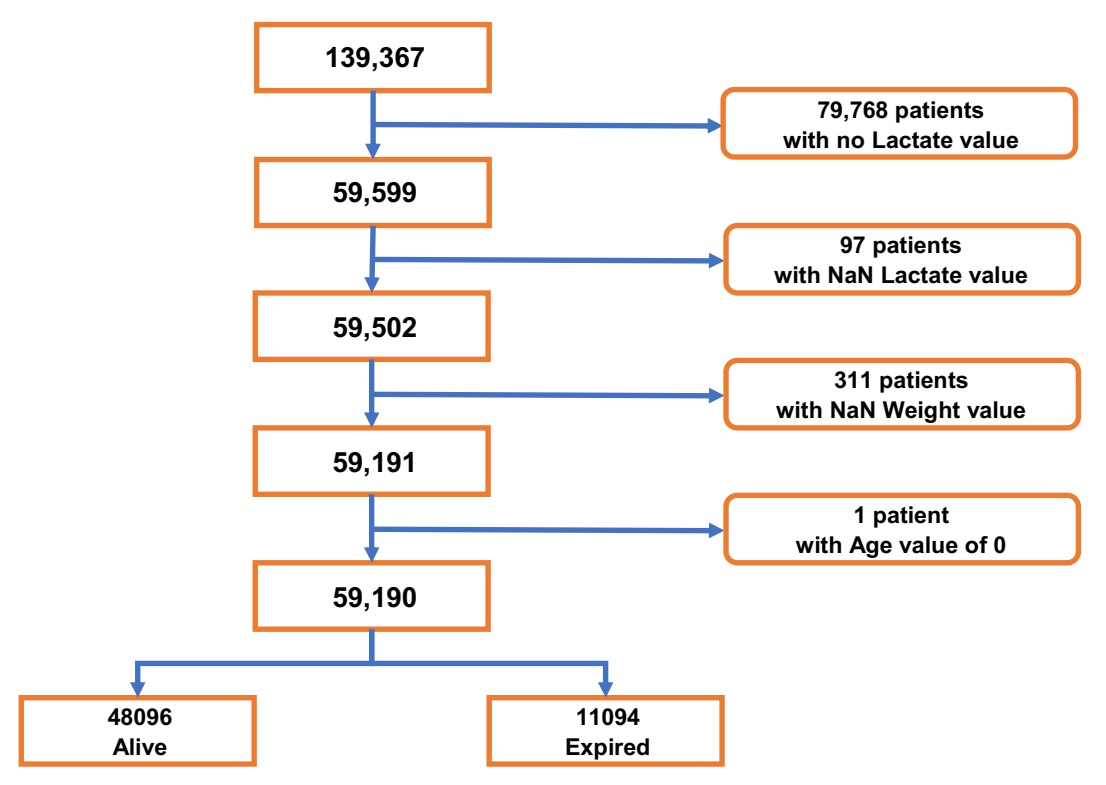
\includegraphics[width=15cm]{fig/chapter3/Cohort Selection Process.jpg}
\caption{Cohort selection process}
\label{fig:cohortselection}
\end{figure}

\subsection{Problems and Limitations}{\label{ssec:limit}}
Obtaining the final cohort was the most time-consuming step of the investigation. The challenges encountered in work are listed as follows: \

\begin{enumerate}[label=\alph*)]
    \item The \acrshort{HUNT} Cloud service was used for implementations and computations of the underway project. The \acrshort{eICU-CRD} has been merely uploaded on and accessible via the Cloud. However, working with a 2.4 GHz Intel Xeon\textregistered{} E5-2680 processor and 16 GB of memory, especially when there is a requirement to separate each patient in order not to bias the training set at the \acrlong{ML} level, could be problematic. It brought about an inability to statistically analyze the \acrshort{eICU} main version in the same manner as performed for the demo version.
    \item A patient with age "0" and some patients with age "\textgreater 89" were found in the database.
    \item For the weight value, we encountered three occasions:
    \begin{enumerate}[label=\arabic*)]
        \item there is value for admission weight, but \acrshort{NaN} for discharge weight, or vice versa.
        \item there is \acrshort{NaN} for both admission and discharge weight.
        \item either of the admission weight or discharge weight was inserted wrong regarding the unit conversion or decimal separator.
    \end{enumerate}
    \item The number of patients with lactate value(s) decreased the number of our cohort rows by more than 57\%.
    \item A patient may be discharged from \acrshort{ICU} with ALIVE status and be discharged from the hospital as EXPIRED, but the opposite is impossible. However, the \acrshort{eICU-CRD} has some of these weird cases.
\end{enumerate}

\subsection{Solutions and Assumptions}
In this section, feasible solutions for the claimed problems in section \ref{ssec:limit} are addressed one by one:

\begin{enumerate}[label=\alph*)]
    \item We focused only on the tables with our designated features. The  \textit{patient} table, the \textit{apachePredVar} table, the \textit{infusionDrug} table, and the \textit{lab} table were the only tables we took into account to create the cohort.
    \item The zero-aged patient was omitted as the information was misleading. The patients who were more than 89 years old, based on the suggestion of the \acrshort{eICU-CRD} website, were assumed to be 90-year-old patients.
    \item In regards to the problem mentioned in the previous section:
    \begin{enumerate}[label=\arabic*)]
        \item we first tried to check whether the weight information is available in the \textit{infusionDrug} table. If not, we replaced the \acrshort{NaN} value with the value of the existing one.
        \item we eliminated the whole row belonging to that specific patient. In case this was the only available weight information, the whole patient's information was disregarded.
        \item dealing with outliers is not a straightforward procedure. As a matter of fact, it is a case that should be treated patient by patient, which is cumbersome. In some cases, it was recognized that one of the values is somehow converted from "lb" to "kg" or a decimal point is missed. Nevertheless, some could be deduced by perception. For instance, a patient cannot get admitted to a hospital with 75 kg and be discharged with 209 kg!
    \end{enumerate}
    \item As described before, we have access to a patient's glucose values through different tables: \textit{apacheApsVar}, \textit{lab}, \textit{medication}, \textit{nurseCharting}, and \textit{treatment}. However, the only table that provides us with the lactate value is the \textit{lab} table. Hence, the number of studied patients for our case could not exceed that. Despite losing nearly 80,000 rows of information, the number of remaining rows is still acceptable and provides sufficient data to analyze.
    \item Mortality status is available in two tables, \textit{patient} and \textit{apachePredVar}. We must check if both tables report the same result.
\end{enumerate}

{\hskip 1em} Ultimately, after applying all the corrections for the plausible problems, should there still be any \acrshort{NaN} value in a row, the entire row would be excluded from the final dataset. \

{\hskip 1em} It is also worth mentioning that one of the features that could have been considered for the cohort was insulin dosage. However, the insulin dosage was not included because the dataset's size was already reduced due to the limitation in the number of lactate values. Instead, the study focused on \acrshort{DM} as an associated feature with glucose and lactate.
